\documentclass[12pt,letterpaper,final]{article}

\usepackage{Sweave}
\usepackage{graphicx}
\usepackage{natbib}
\usepackage{hyperref}
\usepackage{caption}
\usepackage{rotating}
\usepackage{verbatim}
\usepackage{textcomp}
\usepackage{wasysym}

\setlength{\oddsidemargin}{0in}
\setlength{\textwidth}{6.15in}
%\setlength{\topmargin}{0.5in}
\setlength{\textheight}{22cm}
\setlength{\headheight}{0in}
\setlength{\headsep}{0in}
\setlength{\parskip}{5pt plus 2pt minus 3pt}

\def\thefootnote{\fnsymbol{footnote}}
\setcounter{footnote}{1}

\renewcommand{\baselinestretch}{1.2}
\renewcommand{\labelenumi}{(\roman{enumi})}

\renewcommand{\topfraction}{1.0}
\renewcommand{\bottomfraction}{1.0}
\renewcommand{\textfraction}{0.0}
\renewcommand{\floatpagefraction}{1.0}

\newtheorem{definition}{Definition}
\newtheorem{theorem}{Theorem}
\newtheorem{lemma}[theorem]{Lemma}
\newtheorem{claim}[theorem]{Claim}
\newtheorem{fact}[theorem]{Fact}

% to get nice proofs ...
\newcommand{\qedsymb}{\mbox{ }~\hfill~{\rule{2mm}{2mm}}}
\newenvironment{proof}{\begin{trivlist}
\item[\hspace{\labelsep}{\bf\noindent Proof: }]
}{\qedsymb\end{trivlist}}


\newfont{\msymb}{cmsy10 scaled 1000}

\def\nullset{\mbox{\O}}
\def\R{{I\!\!R}}
\def\C{{I\!\!\!\!C}}
\def\N{{I\!\!N}}

\def\P{\mbox{\msymb P}}


%\parskip 0.1in
\pagenumbering{arabic}    %  Start using 1,2,... as page numbers.
\pagestyle{plain}         %  Page numbers in middle bottom of page.
%\setcounter{page}{80}  % XXXXXXXXXXXXXXXXX
%\setcounter{theorem}{5} % XXXXXXXXXXXXXXXXX
%\setcounter{definition}{10} % XXXXXXXXXXXXXXXXX

\parindent 0in


\begin{document}

\Sconcordance{concordance:rnw_template.tex:rnw_template.Rnw:%
1 98 1 1 7 6 1 1 5 1 2 14 1 1 2 5 0 1 2 6 1 1 10 13 0 1 2 24 1 1 3 2 0 %
2 2 1 4 3 0 1 5 4 0 1 4 3 0 1 7 10 0 1 2 21 1 1 9 12 0 1 2 24 1 1 2 1 0 %
1 1 2 3 5 0 1 2 25 1}


\begin{table}\centering
\begin{tabular*}{6.15in}{@{\extracolsep{\fill}}|llr|} \hline
RNW Template File & \hspace*{0.5 in} & Fall 2019 \\
 & & \\
\multicolumn{3}{|c|}{
{\bf Name:} Michael Huber} \\
 & & \\
\multicolumn{3}{|c|}{
{\bf Submission Date:} 10/17/2019} \\
 & & \\
\multicolumn{3}{|c|}{
<Document Information> (10/02/2019)} \\
 & & \\
\multicolumn{3}{|c|}{
45 Points --- Due Friday 10/18/2019 (via Canvas by 11:59pm)} \\
\hline
\end{tabular*}
\end{table}


~ \newpage

\begin{enumerate}

\item \underline{\bf Question 1:}
<description of question 1>


\begin{enumerate}
\item (1 Point) Load all required R packages to answer this question. Show your R code.






\item (1 Point) <first requirement with code>

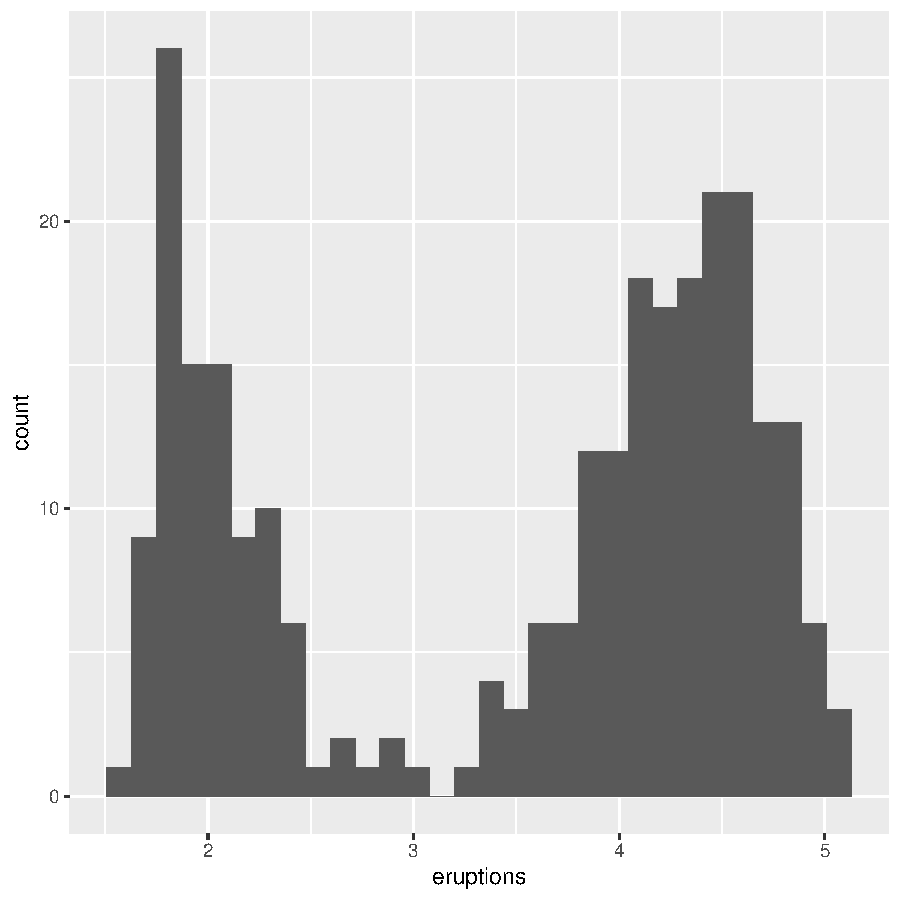
\includegraphics{rnw_template-002}



\underline{Answer:}
\begin{itemize}
\item <Answer Part 1>
\item <Answer Part 2>
\end{itemize}





\item (1 Point) Repeat (b) from above, now using the {\it hist} function from baseR.

\begin{Schunk}
\begin{Sinput}
> hist(faithful$eruptions)
\end{Sinput}
\end{Schunk}
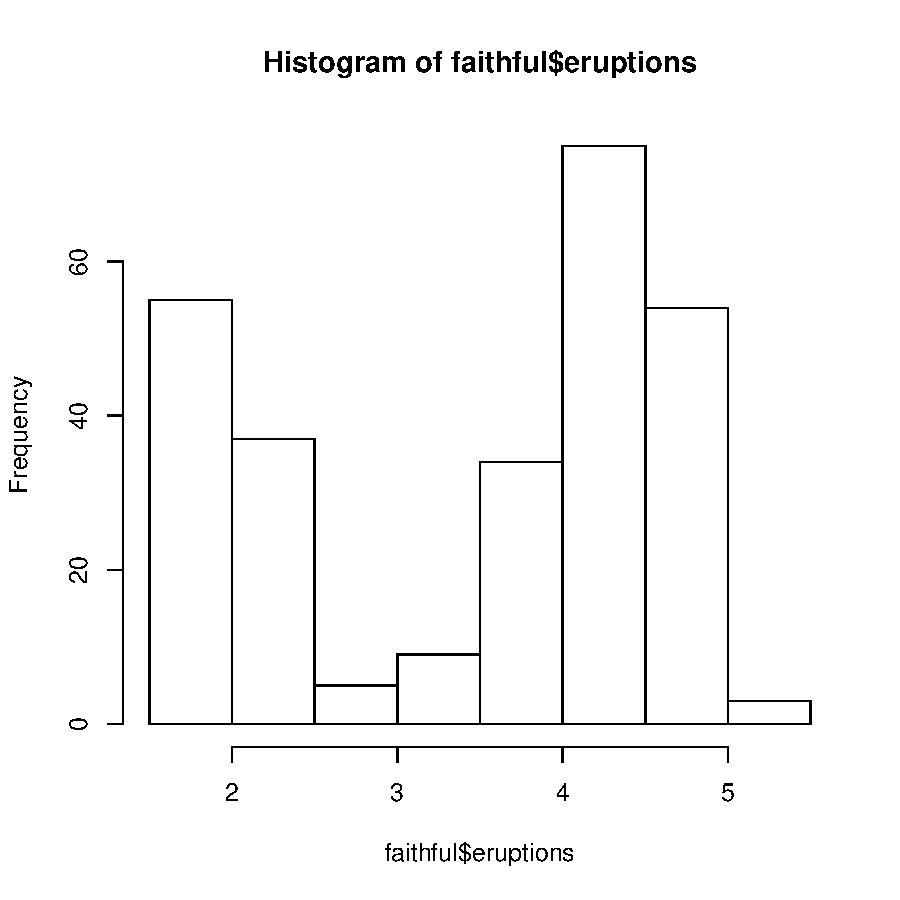
\includegraphics{rnw_template-003}





\item (3 Points) Repeat (c) from above, now using the {\it hist} function from baseR.

\begin{Schunk}
\begin{Sinput}
> hist(faithful$eruptions,
+      breaks = seq(1, 6, .5),
+      xlab = "Eruption Time in Minutes",
+      ylab = "Count of Eruptions",
+      main = "Old Faithful Eruption Data Histogram",
+      col = "light blue",
+      las = 1,
+      ylim = c(0, 100),
+      xlim = c(1, 6))
\end{Sinput}
\end{Schunk}
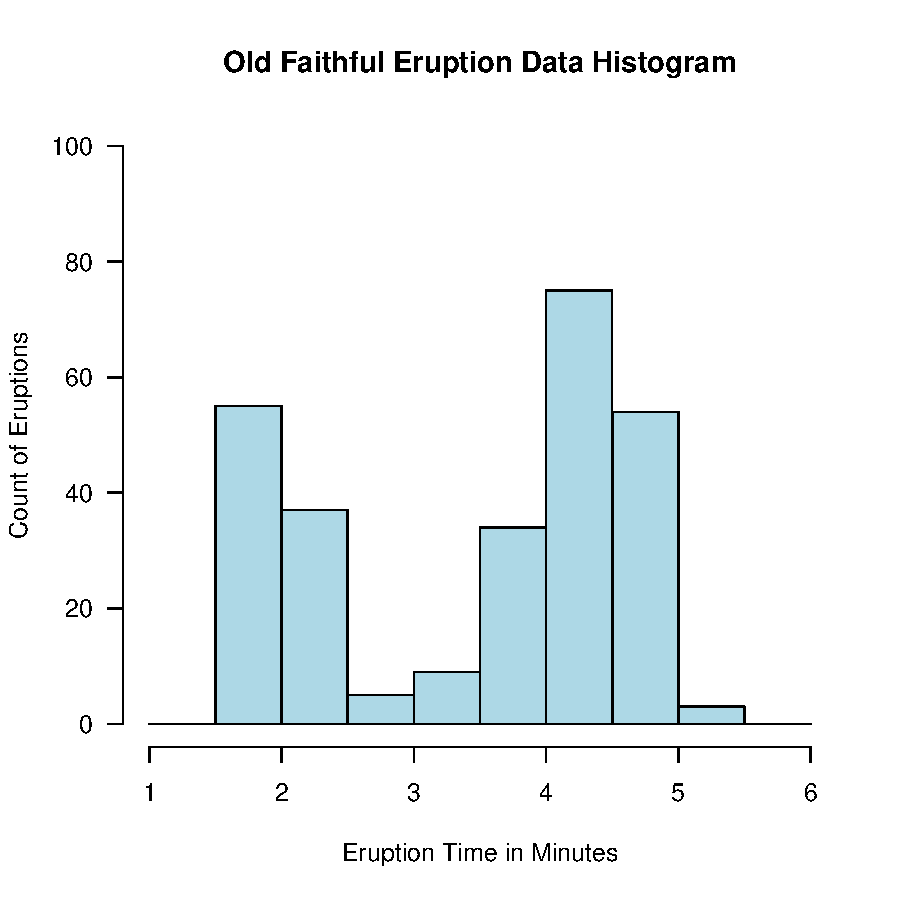
\includegraphics{rnw_template-004}

\underline{Answer:}
\begin{itemize}
\item <Answer Part 1>
\item <Answer Part 2>
\end{itemize}


\end{enumerate}


\newpage


\item \underline{\bf Question 2:}
<Description of Question 2>


\begin{enumerate}
\item (6 Points) Recreate the graphs (and layout) below using baseR.
Use a ruler to  check that the width and height proportions in your graphs
match the ones I have used. I worked with integer multiples!
Include your R code and the resulting graphs.
Hint: You can create a new line via \verb|\n| without any extra spaces before/after \verb|\n|.

\begin{Schunk}
\begin{Sinput}
> grid <- matrix(c(1, 1, 1, 2, 2, 3, 3, 3, 4, 4), 
+               nrow = 2, ncol = 5, byrow = TRUE)
> layout(grid)
> par(mar = c(4, 3, 4, 2))
> boxplot(geyser$duration,
+         horizontal = TRUE,
+         main = "Old Faithful:\n Duration",
+         ylim = c(0, 6))
> hist(geyser$duration,
+      main = "Old Faithful",
+      xlab = "Duration",
+      ylab = "Count",
+      xlim = c(0, 6))
> boxplot(geyser$waiting,
+         horizontal = TRUE,
+         main = "Old Faithful:\n Waiting",
+         ylim = c(40, 120))
> hist(geyser$waiting,
+      main = "Old Faithful",
+      xlab = "Waiting",
+      ylab = "Count",
+      xlim = c(40, 120),
+      ylim = c(0, 100),
+      breaks = seq(40, 120, by = 10))
\end{Sinput}
\end{Schunk}
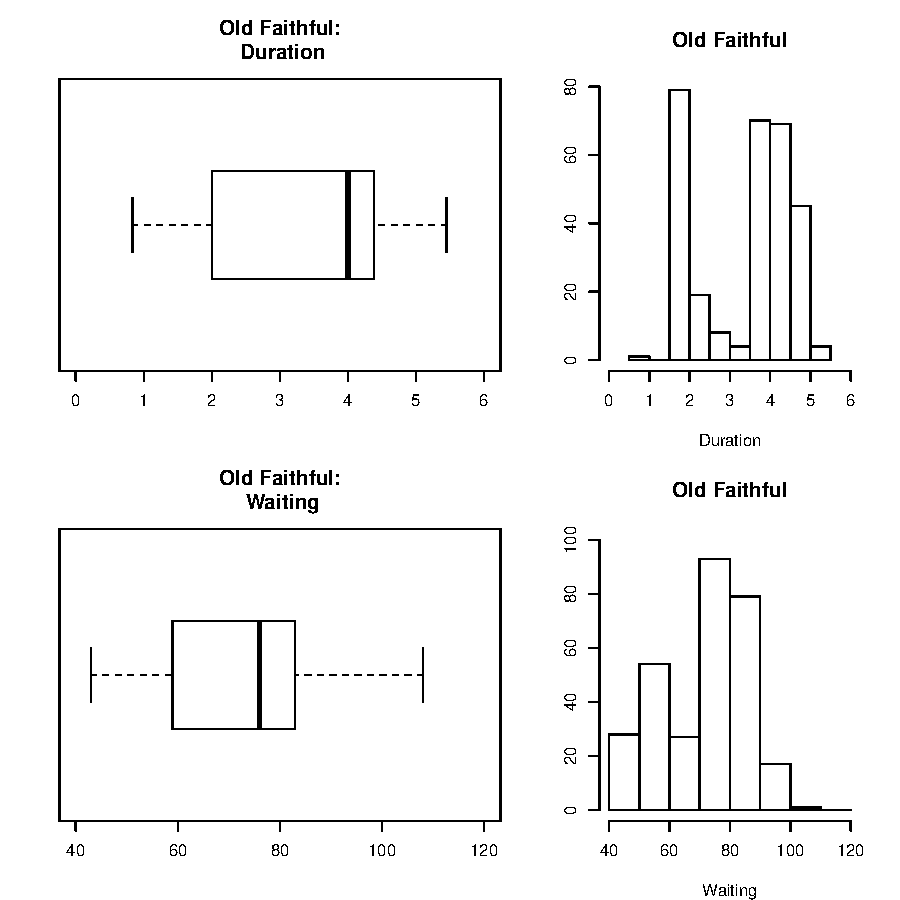
\includegraphics{rnw_template-005}
\underline{Refernces:}
\begin{itemize}
\item https://www.statmethods.net/advgraphs/layout.html
\item https://stackoverflow.com/questions/31319942/change-the-size-of-a-plot-when-plotting-multiple-plots-in-r
\item https://www.youtube.com/watch?v=Z3V4Pbxeahg
\end{itemize}

\begin{figure}[ht]
\centering{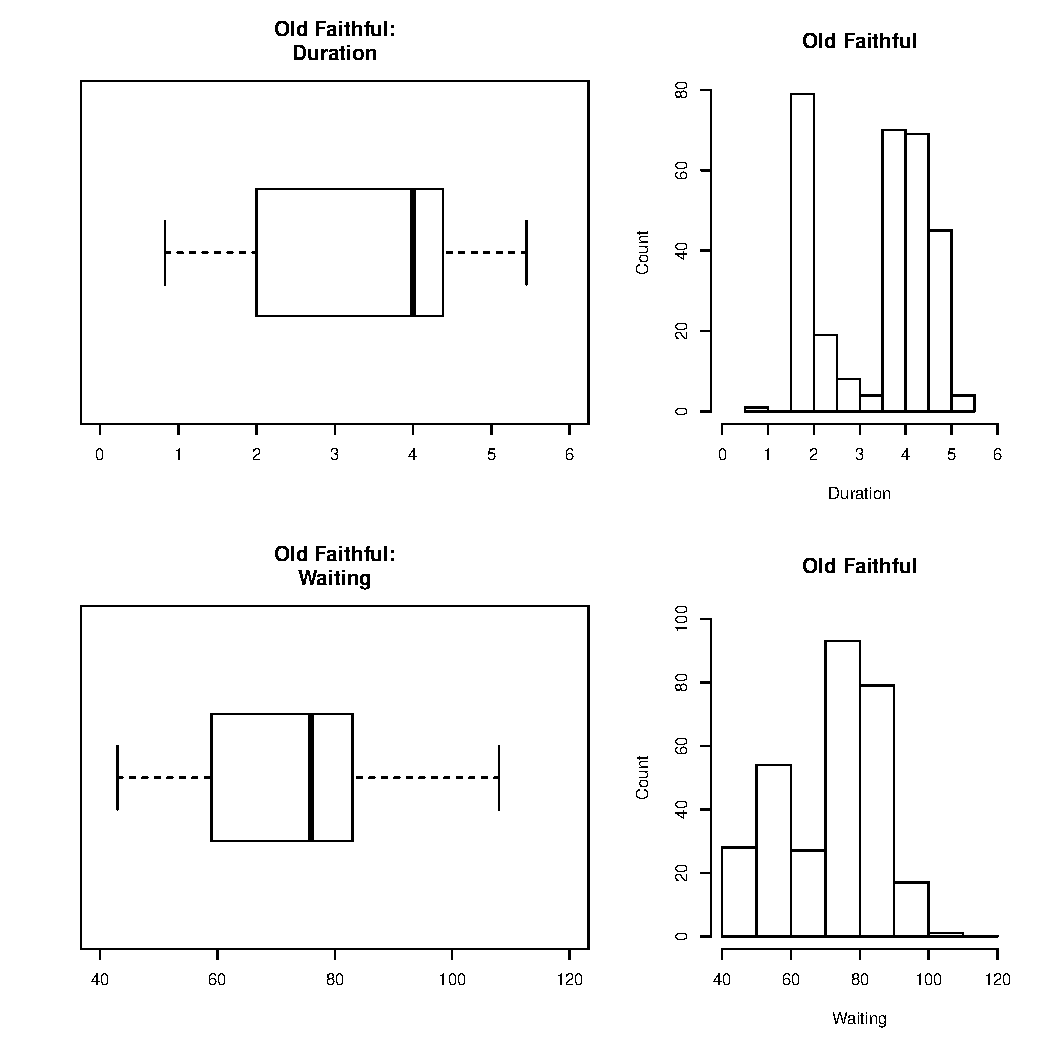
\includegraphics[width=5in]{hw01_q2a.pdf}}
\caption{\label{hw01_q2a}
Graph created with {\it baseR}.
}
\end{figure}



\newpage


\item (2 Points) Recreate the graph below using ggplot2.
Include your R code and the resulting graph.

\begin{Schunk}
\begin{Sinput}
> ggplot(geyser, aes(x=duration, y=waiting)) +
+   geom_point() +
+   xlab("Duration") +
+   ylab("Waiting") +
+   xlim(0, 6) +
+   ylim(40, 120) +
+   ggtitle("Old Faithful Data") +
+   theme(plot.title = element_text(hjust = 0.5))
\end{Sinput}
\end{Schunk}
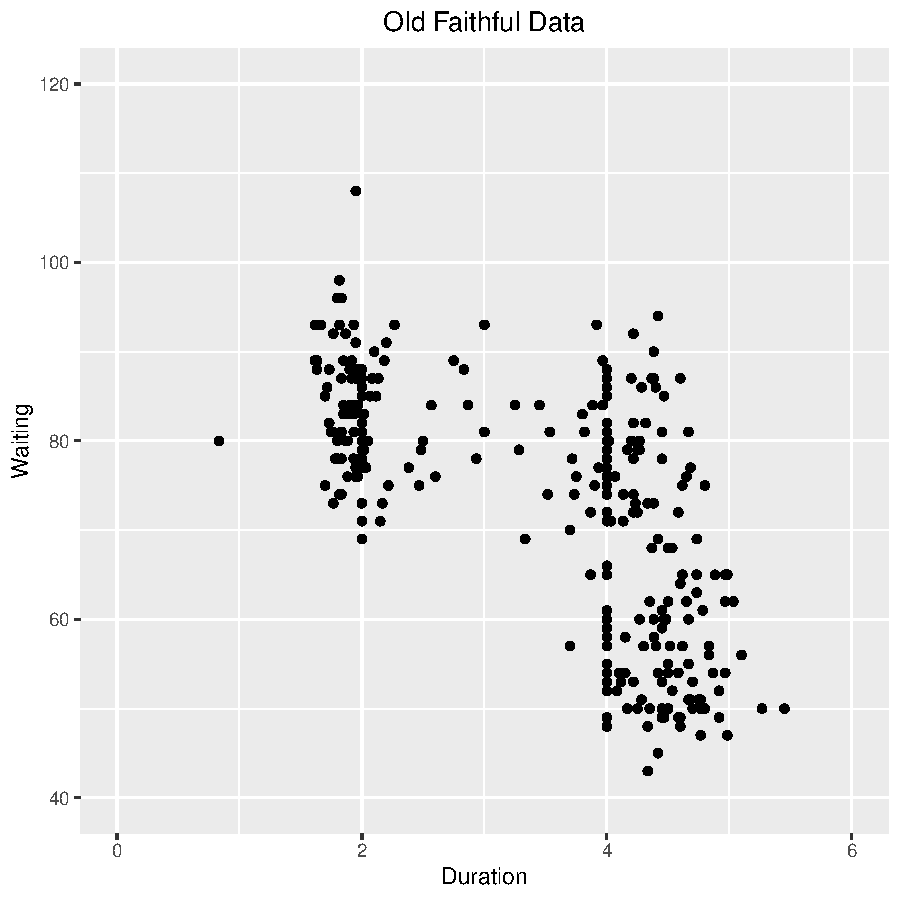
\includegraphics{rnw_template-006}


% Pulls in a pdf document that is in the same directory
\begin{figure}[ht]
\centering{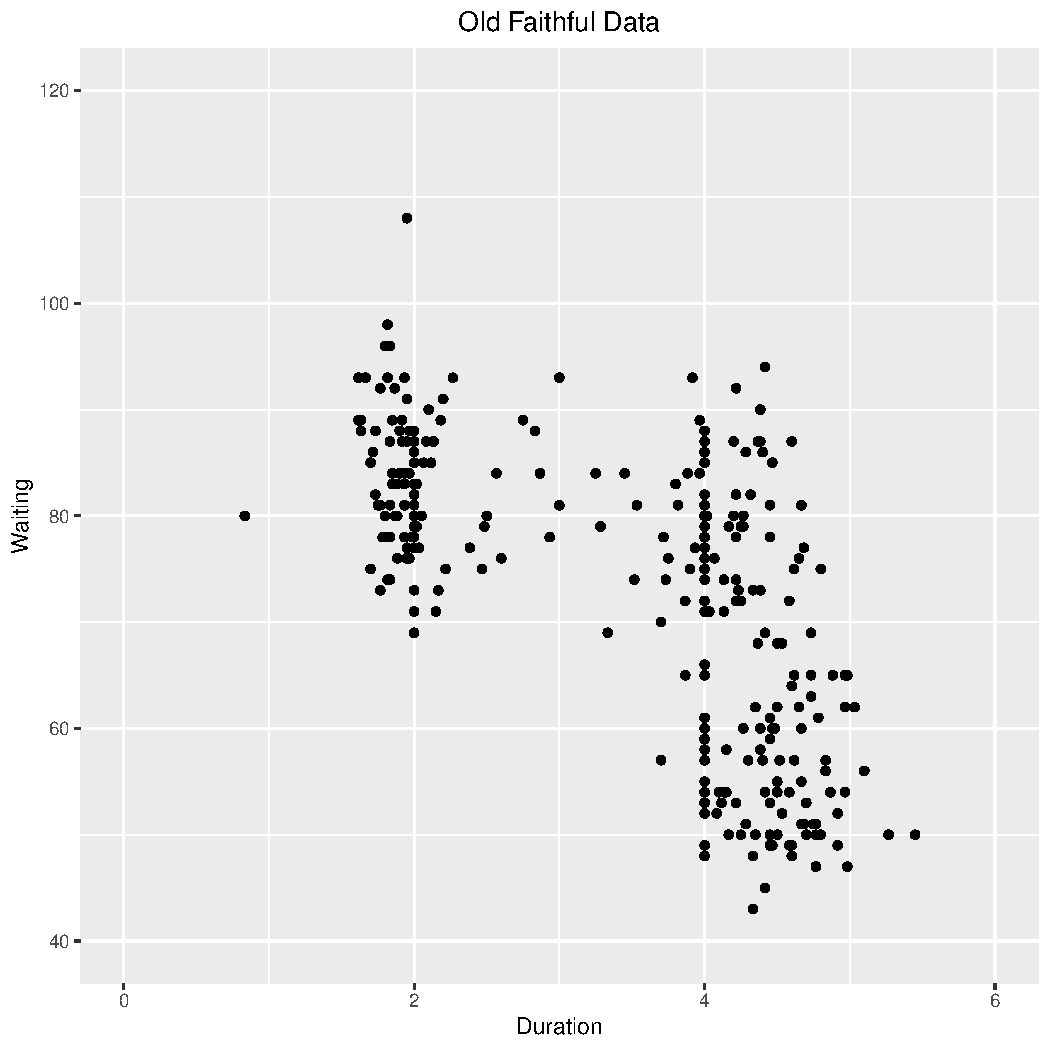
\includegraphics[width=5.0in]{hw01_q2b.pdf}}
\caption{\label{hw01_q2b}
Graph created with {\it ggplot2}.
}
\end{figure}


\newpage


\item (2 Points) Doesn't the scatterplot in (b) above look rather different 
than the scatterplot in Question 1 (j)? Note that the help page for {\it geyser}
states \verb|waiting	 numeric	 Waiting time for this eruption| and \\
\verb|The waiting time was incorrectly described as the time to the next|
\verb|eruption in the original files, and corrected for MASS version 7.3-30.| \\
Use this information to create a basic scatterplot 
for the {\it geyser} data that matches the overall 
appearance in Question 1 (j). 
Include your R code and the resulting graph.
No need to refine this scatterplot.

\begin{Schunk}
\begin{Sinput}
> duration <- geyser$duration[1:298]
> waiting <- geyser$waiting[2:299]
> df <- data.frame(duration, waiting)
> ggplot(df, aes(x = duration, y = waiting )) + 
+          geom_point()
\end{Sinput}
\end{Schunk}
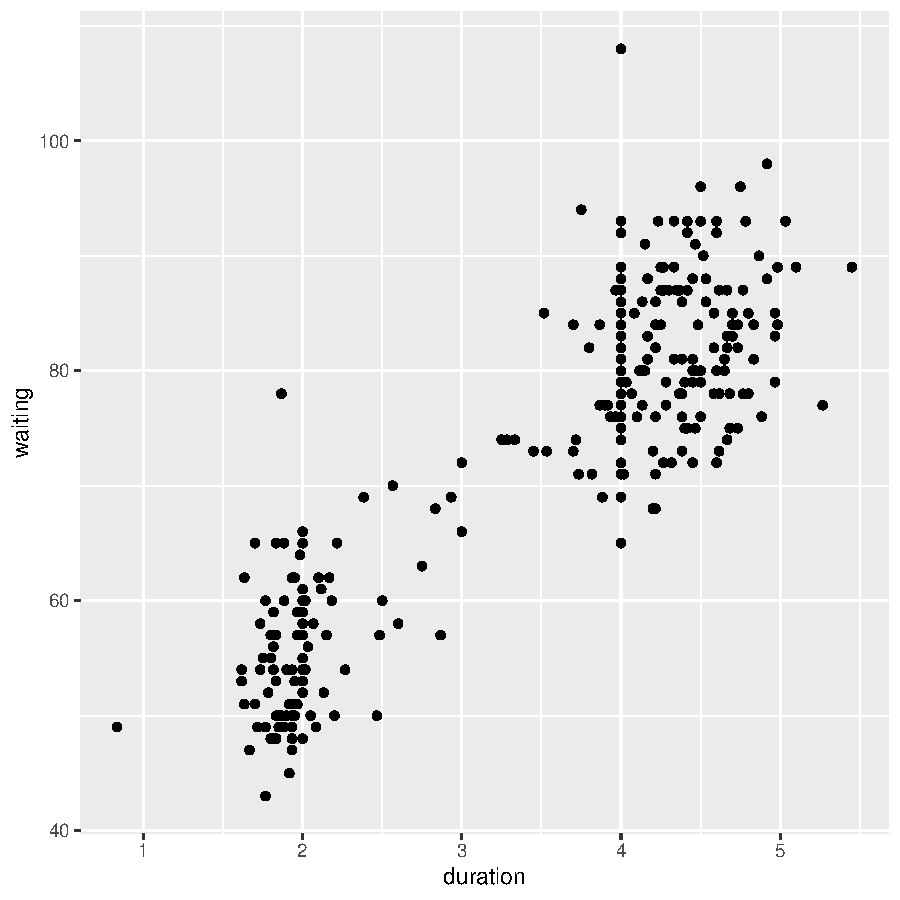
\includegraphics{rnw_template-007}

\underline{Answer:} 
The geyser data appears to have a negative correlation with three clusters where the faithful data has a positive correlation with 2 clusters.


\end{enumerate}

\end{enumerate}


\newpage


\noindent{\Large \bf General Instructions}~\\

\begin{enumerate}

\item <Instruction 1>

\item <Instruction 2>

\end{enumerate}


\end{document}

